% Created by tikzDevice version 0.7.0 on 2014-04-27 12:59:54
% !TEX encoding = UTF-8 Unicode
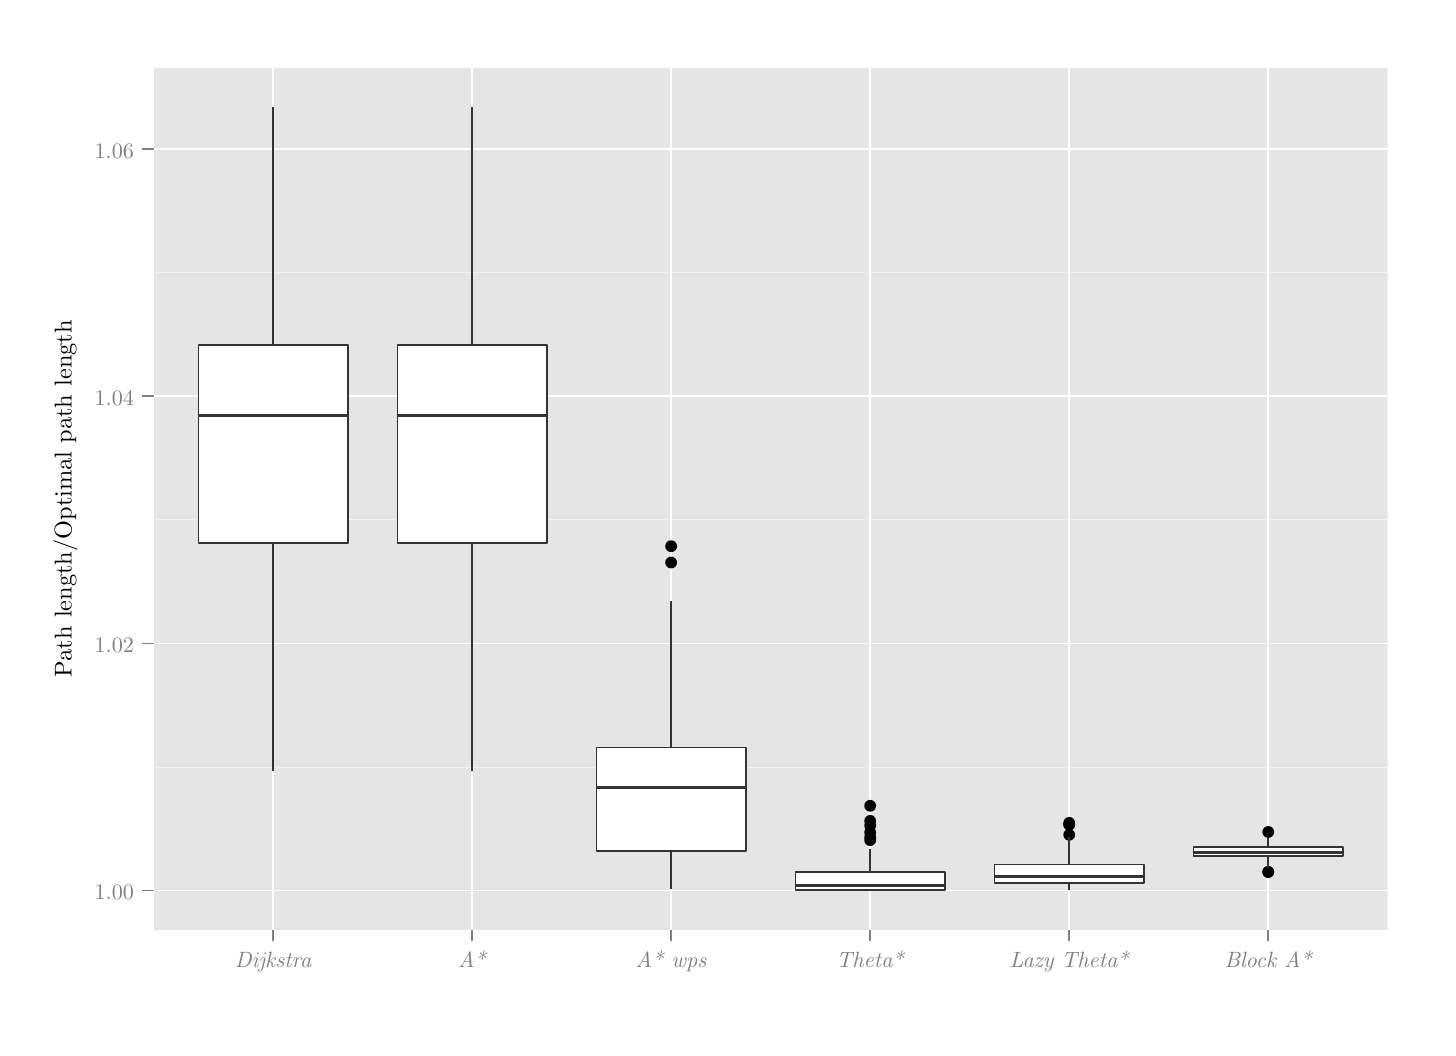
\begin{tikzpicture}[x=1pt,y=1pt]
\definecolor[named]{fillColor}{rgb}{1.00,1.00,1.00}
\path[use as bounding box,fill=fillColor,fill opacity=0.00] (0,0) rectangle (505.89,361.35);
\begin{scope}
\path[clip] (  0.00,  0.00) rectangle (505.89,361.35);
\definecolor[named]{drawColor}{rgb}{1.00,1.00,1.00}
\definecolor[named]{fillColor}{rgb}{1.00,1.00,1.00}

\path[draw=drawColor,line width= 0.6pt,line join=round,line cap=round,fill=fillColor] (  0.00, -0.00) rectangle (505.89,361.35);
\end{scope}
\begin{scope}
\path[clip] ( 45.51, 35.41) rectangle (491.44,346.90);
\definecolor[named]{fillColor}{rgb}{0.90,0.90,0.90}

\path[fill=fillColor] ( 45.51, 35.41) rectangle (491.44,346.90);
\definecolor[named]{drawColor}{rgb}{0.95,0.95,0.95}

\path[draw=drawColor,line width= 0.3pt,line join=round] ( 45.51, 94.21) --
	(491.44, 94.21);

\path[draw=drawColor,line width= 0.3pt,line join=round] ( 45.51,183.50) --
	(491.44,183.50);

\path[draw=drawColor,line width= 0.3pt,line join=round] ( 45.51,272.78) --
	(491.44,272.78);
\definecolor[named]{drawColor}{rgb}{1.00,1.00,1.00}

\path[draw=drawColor,line width= 0.6pt,line join=round] ( 45.51, 49.57) --
	(491.44, 49.57);

\path[draw=drawColor,line width= 0.6pt,line join=round] ( 45.51,138.85) --
	(491.44,138.85);

\path[draw=drawColor,line width= 0.6pt,line join=round] ( 45.51,228.14) --
	(491.44,228.14);

\path[draw=drawColor,line width= 0.6pt,line join=round] ( 45.51,317.43) --
	(491.44,317.43);

\path[draw=drawColor,line width= 0.6pt,line join=round] ( 88.66, 35.41) --
	( 88.66,346.90);

\path[draw=drawColor,line width= 0.6pt,line join=round] (160.58, 35.41) --
	(160.58,346.90);

\path[draw=drawColor,line width= 0.6pt,line join=round] (232.51, 35.41) --
	(232.51,346.90);

\path[draw=drawColor,line width= 0.6pt,line join=round] (304.43, 35.41) --
	(304.43,346.90);

\path[draw=drawColor,line width= 0.6pt,line join=round] (376.36, 35.41) --
	(376.36,346.90);

\path[draw=drawColor,line width= 0.6pt,line join=round] (448.28, 35.41) --
	(448.28,346.90);
\definecolor[named]{drawColor}{rgb}{0.20,0.20,0.20}
\definecolor[named]{fillColor}{rgb}{0.20,0.20,0.20}

\path[draw=drawColor,line width= 0.6pt,line join=round,fill=fillColor] ( 88.66,246.62) -- ( 88.66,332.74);

\path[draw=drawColor,line width= 0.6pt,line join=round,fill=fillColor] ( 88.66,175.23) -- ( 88.66, 92.65);
\definecolor[named]{fillColor}{rgb}{1.00,1.00,1.00}

\path[draw=drawColor,line width= 0.6pt,line join=round,line cap=round,fill=fillColor] ( 61.69,246.62) --
	( 61.69,175.23) --
	(115.63,175.23) --
	(115.63,246.62) --
	( 61.69,246.62) --
	cycle;
\definecolor[named]{fillColor}{rgb}{0.20,0.20,0.20}

\path[draw=drawColor,line width= 1.1pt,line join=round,fill=fillColor] ( 61.69,221.20) -- (115.63,221.20);

\path[draw=drawColor,line width= 0.6pt,line join=round,fill=fillColor] (160.58,246.62) -- (160.58,332.74);

\path[draw=drawColor,line width= 0.6pt,line join=round,fill=fillColor] (160.58,175.23) -- (160.58, 92.65);
\definecolor[named]{fillColor}{rgb}{1.00,1.00,1.00}

\path[draw=drawColor,line width= 0.6pt,line join=round,line cap=round,fill=fillColor] (133.61,246.62) --
	(133.61,175.23) --
	(187.56,175.23) --
	(187.56,246.62) --
	(133.61,246.62) --
	cycle;
\definecolor[named]{fillColor}{rgb}{0.20,0.20,0.20}

\path[draw=drawColor,line width= 1.1pt,line join=round,fill=fillColor] (133.61,221.20) -- (187.56,221.20);
\definecolor[named]{fillColor}{rgb}{0.00,0.00,0.00}

\path[fill=fillColor] (232.51,173.98) circle (  2.13);

\path[fill=fillColor] (232.51,168.07) circle (  2.13);
\definecolor[named]{fillColor}{rgb}{0.20,0.20,0.20}

\path[draw=drawColor,line width= 0.6pt,line join=round,fill=fillColor] (232.51,101.24) -- (232.51,154.28);

\path[draw=drawColor,line width= 0.6pt,line join=round,fill=fillColor] (232.51, 63.77) -- (232.51, 49.99);
\definecolor[named]{fillColor}{rgb}{1.00,1.00,1.00}

\path[draw=drawColor,line width= 0.6pt,line join=round,line cap=round,fill=fillColor] (205.54,101.24) --
	(205.54, 63.77) --
	(259.48, 63.77) --
	(259.48,101.24) --
	(205.54,101.24) --
	cycle;
\definecolor[named]{fillColor}{rgb}{0.20,0.20,0.20}

\path[draw=drawColor,line width= 1.1pt,line join=round,fill=fillColor] (205.54, 86.70) -- (259.48, 86.70);
\definecolor[named]{fillColor}{rgb}{0.00,0.00,0.00}

\path[fill=fillColor] (304.43, 80.18) circle (  2.13);

\path[fill=fillColor] (304.43, 74.72) circle (  2.13);

\path[fill=fillColor] (304.43, 67.78) circle (  2.13);

\path[fill=fillColor] (304.43, 70.59) circle (  2.13);

\path[fill=fillColor] (304.43, 73.04) circle (  2.13);

\path[fill=fillColor] (304.43, 68.80) circle (  2.13);
\definecolor[named]{fillColor}{rgb}{0.20,0.20,0.20}

\path[draw=drawColor,line width= 0.6pt,line join=round,fill=fillColor] (304.43, 56.15) -- (304.43, 64.69);

\path[draw=drawColor,line width= 0.6pt,line join=round,fill=fillColor] (304.43, 49.63) -- (304.43, 49.57);
\definecolor[named]{fillColor}{rgb}{1.00,1.00,1.00}

\path[draw=drawColor,line width= 0.6pt,line join=round,line cap=round,fill=fillColor] (277.46, 56.15) --
	(277.46, 49.63) --
	(331.40, 49.63) --
	(331.40, 56.15) --
	(277.46, 56.15) --
	cycle;
\definecolor[named]{fillColor}{rgb}{0.20,0.20,0.20}

\path[draw=drawColor,line width= 1.1pt,line join=round,fill=fillColor] (277.46, 51.37) -- (331.40, 51.37);
\definecolor[named]{fillColor}{rgb}{0.00,0.00,0.00}

\path[fill=fillColor] (376.36, 74.00) circle (  2.13);

\path[fill=fillColor] (376.36, 69.70) circle (  2.13);

\path[fill=fillColor] (376.36, 73.32) circle (  2.13);

\path[fill=fillColor] (376.36, 73.52) circle (  2.13);
\definecolor[named]{fillColor}{rgb}{0.20,0.20,0.20}

\path[draw=drawColor,line width= 0.6pt,line join=round,fill=fillColor] (376.36, 59.00) -- (376.36, 68.94);

\path[draw=drawColor,line width= 0.6pt,line join=round,fill=fillColor] (376.36, 52.30) -- (376.36, 49.57);
\definecolor[named]{fillColor}{rgb}{1.00,1.00,1.00}

\path[draw=drawColor,line width= 0.6pt,line join=round,line cap=round,fill=fillColor] (349.39, 59.00) --
	(349.39, 52.30) --
	(403.33, 52.30) --
	(403.33, 59.00) --
	(349.39, 59.00) --
	cycle;
\definecolor[named]{fillColor}{rgb}{0.20,0.20,0.20}

\path[draw=drawColor,line width= 1.1pt,line join=round,fill=fillColor] (349.39, 54.46) -- (403.33, 54.46);
\definecolor[named]{fillColor}{rgb}{0.00,0.00,0.00}

\path[fill=fillColor] (448.28, 70.72) circle (  2.13);

\path[fill=fillColor] (448.28, 56.25) circle (  2.13);

\path[fill=fillColor] (448.28, 56.29) circle (  2.13);
\definecolor[named]{fillColor}{rgb}{0.20,0.20,0.20}

\path[draw=drawColor,line width= 0.6pt,line join=round,fill=fillColor] (448.28, 65.29) -- (448.28, 68.51);

\path[draw=drawColor,line width= 0.6pt,line join=round,fill=fillColor] (448.28, 62.08) -- (448.28, 57.80);
\definecolor[named]{fillColor}{rgb}{1.00,1.00,1.00}

\path[draw=drawColor,line width= 0.6pt,line join=round,line cap=round,fill=fillColor] (421.31, 65.29) --
	(421.31, 62.08) --
	(475.25, 62.08) --
	(475.25, 65.29) --
	(421.31, 65.29) --
	cycle;
\definecolor[named]{fillColor}{rgb}{0.20,0.20,0.20}

\path[draw=drawColor,line width= 1.1pt,line join=round,fill=fillColor] (421.31, 63.44) -- (475.25, 63.44);
\end{scope}
\begin{scope}
\path[clip] (  0.00,  0.00) rectangle (505.89,361.35);
\definecolor[named]{drawColor}{rgb}{0.50,0.50,0.50}

\node[text=drawColor,anchor=base east,inner sep=0pt, outer sep=0pt, scale=  0.80] at ( 38.39, 46.26) {1.00};

\node[text=drawColor,anchor=base east,inner sep=0pt, outer sep=0pt, scale=  0.80] at ( 38.39,135.55) {1.02};

\node[text=drawColor,anchor=base east,inner sep=0pt, outer sep=0pt, scale=  0.80] at ( 38.39,224.83) {1.04};

\node[text=drawColor,anchor=base east,inner sep=0pt, outer sep=0pt, scale=  0.80] at ( 38.39,314.12) {1.06};
\end{scope}
\begin{scope}
\path[clip] (  0.00,  0.00) rectangle (505.89,361.35);
\definecolor[named]{drawColor}{rgb}{0.50,0.50,0.50}

\path[draw=drawColor,line width= 0.6pt,line join=round] ( 41.24, 49.57) --
	( 45.51, 49.57);

\path[draw=drawColor,line width= 0.6pt,line join=round] ( 41.24,138.85) --
	( 45.51,138.85);

\path[draw=drawColor,line width= 0.6pt,line join=round] ( 41.24,228.14) --
	( 45.51,228.14);

\path[draw=drawColor,line width= 0.6pt,line join=round] ( 41.24,317.43) --
	( 45.51,317.43);
\end{scope}
\begin{scope}
\path[clip] (  0.00,  0.00) rectangle (505.89,361.35);
\definecolor[named]{drawColor}{rgb}{0.50,0.50,0.50}

\path[draw=drawColor,line width= 0.6pt,line join=round] ( 88.66, 31.14) --
	( 88.66, 35.41);

\path[draw=drawColor,line width= 0.6pt,line join=round] (160.58, 31.14) --
	(160.58, 35.41);

\path[draw=drawColor,line width= 0.6pt,line join=round] (232.51, 31.14) --
	(232.51, 35.41);

\path[draw=drawColor,line width= 0.6pt,line join=round] (304.43, 31.14) --
	(304.43, 35.41);

\path[draw=drawColor,line width= 0.6pt,line join=round] (376.36, 31.14) --
	(376.36, 35.41);

\path[draw=drawColor,line width= 0.6pt,line join=round] (448.28, 31.14) --
	(448.28, 35.41);
\end{scope}
\begin{scope}
\path[clip] (  0.00,  0.00) rectangle (505.89,361.35);
\definecolor[named]{drawColor}{rgb}{0.50,0.50,0.50}

\node[text=drawColor,anchor=base,inner sep=0pt, outer sep=0pt, scale=  0.80] at ( 88.66, 21.69) {{\em Dijkstra}};

\node[text=drawColor,anchor=base,inner sep=0pt, outer sep=0pt, scale=  0.80] at (160.58, 21.69) {{\em A*}};

\node[text=drawColor,anchor=base,inner sep=0pt, outer sep=0pt, scale=  0.80] at (232.51, 21.69) {{\em A* wps}};

\node[text=drawColor,anchor=base,inner sep=0pt, outer sep=0pt, scale=  0.80] at (304.43, 21.69) {{\em Theta*}};

\node[text=drawColor,anchor=base,inner sep=0pt, outer sep=0pt, scale=  0.80] at (376.36, 21.69) {{\em Lazy Theta*}};

\node[text=drawColor,anchor=base,inner sep=0pt, outer sep=0pt, scale=  0.80] at (448.28, 21.69) {{\em Block A*}};
\end{scope}
\begin{scope}
\path[clip] (  0.00,  0.00) rectangle (505.89,361.35);
\definecolor[named]{drawColor}{rgb}{0.00,0.00,0.00}

\node[text=drawColor,rotate= 90.00,anchor=base,inner sep=0pt, outer sep=0pt, scale=  0.88] at ( 15.90,191.15) {Path length/Optimal path length};
\end{scope}
\end{tikzpicture}
